\section{AlexNet}\label{alexnet}
AlexNet è una CNN creata tra il 2011 e il 2012 da Alex Krizhevsky, in collaborazione con Ilya Sutskever e Geoffrey Hinton \cite{alexnet}. La vittoria di AlexNet nella ImageNet Large Scale Visual Recognition Challenge (ILSVRC) \cite{imagenet2012}, ottenuta con un netto distacco nei confronti degli altri concorrenti, ha segnato l'inizio dell'enorme successo ottenuto dalle reti neurali profonde in svariati domini di applicazione \cite{historydl}

Il risultato principale di AlexNet, così come dichiarato dai suoi creatori nell'articolo originale, è il fatto che la profondità del modello è stato essenziale per conferirgli prestazioni così alte. L'alto costo computazionale dell'addestramento di AlexNet, reso oneroso appunto dalla profondità del modello (e quindi dal grande numero di parametri - circa 62.3 milioni) è stato affrontato con l'impiego di schede grafiche (GPU), che cominciavano in quegli anni a raggiungere notevoli potenze di calcolo.

\subsection{Architettura di AlexNet}
L'architettura di AlexNet è riportata schematicamente nella figura \ref{arc_alexnet} e con maggiore dettaglio in tabella \ref{tab_arc_alexnet}.
La rete accetta in input immagini $227\times 227$. Essa si compone di otto layer con parametri - cinque convoluzionali e tre completamente connessi. L'output dell'ultimo layer completamente connesso passa per un softmax layer a 1000 vie, il quale fornisce la distribuzione di probabilità per le 1000 classi del dataset ImageNet.

Tra ognuno degli otto strati parametrizzati sono interposti alcuni strati intermedi: ReLU layer, Local Response Normalization layer, Max Pooling layer, Dropout layer. Ognuno di questi sarà analizzato in maggiore dettaglio nei paragrafi successivi.

\begin{figure}[h]
\centering
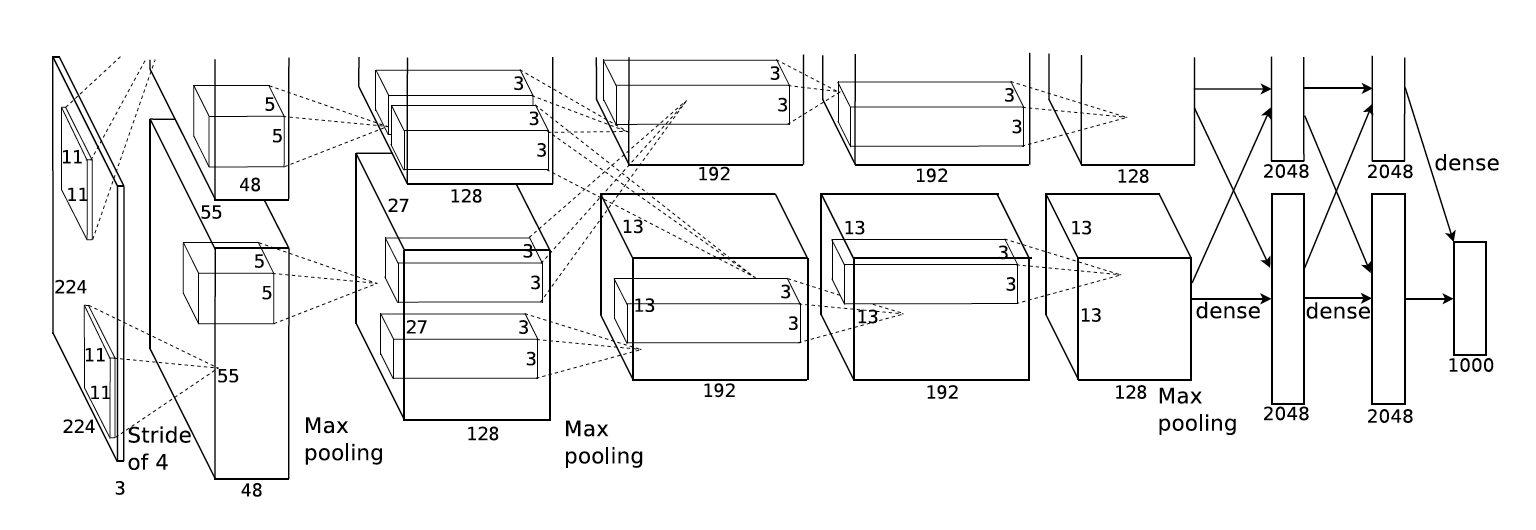
\includegraphics[width=\textwidth ,keepaspectratio]{arc_alexnet}
\caption{Architettura originale di AlexNet \cite{alexnet}}
\label{arc_alexnet}
\end{figure}

Come si evince dalla figura \ref{arc_alexnet}, la rete è composta da due "\textit{pipeline}" parallele. Si scelse infatti di "estendere" la rete su due GPU NVIDIA\textsuperscript{\textregistered} GeForce\textsuperscript{\textregistered} GTX 580 3GB in fase di training, per raddoppiare la memoria massima disponibile (6GB in totale) per conservare la rete e i suoi parametri.

Queste GPU si prestano bene a lavorare in parallelo, poiché possono leggere e scrivere l'una sull'altra direttamente, senza passare dalla memoria della macchina host. Lo schema di parallelizzazione a due vie prevede che su ogni GPU risieda la metà dei kernel (o dei neuroni) di ciascuno strato parametrizzato. Le GPU possono comunicare tra loro solo in certi strati. In particolare, i kernel del layer convoluzionale 1 e 3 hanno in input l'intero output volume rispettivamente del layer di input e del layer convoluzionale 2, mentre i kernel dei rimanenti strati convoluzionali hanno in input la sola metà dell'output volume presente nella stessa GPU (\textit{grouped convolution}\footnote{La scelta di questo pattern di connettività fra le due GPU parallele è il risultato di un problema di cross-validation.}.\\

Sono di seguito passate in rassegna le principali scelte architetturali introdotte in AlexNet, ed alcuni dettagli relativi al suo addestramento.

\subsection*{Funzione di attivazione ReLU}
Dopo ogni strato parametrizzato, i valori delle attivazioni sono passati alla funzione attivatrice "rettificatore": $f(x)=x^{+}=\max(0,x)$ \cite{nairhinton}. Questa funzione attivatrice non-lineare e non soggetta a saturazione permette un addestramento molto più veloce delle reti convoluzionali profonde, in confronto a funzioni attivatrici fino ad allora più utilizzate come la funzione sigmoidea $f(x)=(1+\exp^{-x})^{-1}$ e la funzione tangente iperbolica $f(x)=\tanh(x)$.

\subsection*{Local Response Normalization}
È stato verificato che la seguente normalizzazione delle attivazioni, \textit{Local Response Normalization}, aumenta lievemente la capacità di generalizzazione del modello:

\[b_{x,y}^{i}=a_{x,y}^{i}/\left(k+\alpha \sum_{j=\max(0,i-n/2)}^{\min(N-1,i+n/2)}(a_{x,y}^{j})^{2}\right)^{\beta}\]

dove $a_{x,y}^{i}$ è l'attivazione del neurone ottenuto applicando il kernel $i$-esimo alla posizione $(x,y)$ e applicando in seguito la funzione ReLU, $b_{x,y}^{i}$ l'attivazione normalizzata, $N$ il numero totale di kernel del layer corrente, $k, n, \alpha, \beta$ sono iperparametri; sono stati usati i valori $k=2, n=5, \alpha=10^{-4}, \beta=0.75$.

Questa normalizzazione è adoperata solamente nel primo e nel secondo layer convoluzionale.

\subsection*{Overlapping Max Pooling}
La funzione di max pooling in AlexNet è stata caratterizzata dalla scelta di una dimensione del filtro di pooling $3\times 3$ e uno stride di $2$. È stato osservato durante la fase di training che questa funzione di \textit{max pooling con sovrapposizione} ha attenuato lievemente l'\textit{overfitting} della rete.

\subsection*{Data Augmentation}
Una delle difficoltà che si incontrano spesso quando si vuole addestrare una rete neurale con moltissimi parametri avendo a disposizione un dataset relativamente piccolo è il rischio del sovradattamento (\textit{overfitting}) della rete al training set, che compromette anche seriamente le prestazioni della rete quando le vengono presentati nuovi dati.
In AlexNet l'overfitting è stato ridotto grazie a tecniche di \textit{data augmentation}. In particolare, dopo aver ridimensionato a $256\times 256$ tutte le immagini del training set, quest'ultimo è stato "arricchito" con le seguenti immagini:
\begin{itemize}
\item Estrazione casuale di ritagli $224\times 224$ dalle immagini
\item Riflessione orizzontale ("a specchio") delle immagini
\item Somma di un'immagine e le sue componenti principali (PCA)\footnote{L'\textit{analisi delle componenti principali} (PCA, principal component analysis) è una tecnica per la semplificazione dei dati utilizzata nell'ambito della statistica multivariata. In questa sede ci limitiamo a specificare che il suo utilizzo nell'ambito della data augmentation è di evidenziare una importante proprietà delle immagini naturali, e cioè che l'identità di un oggetto è invariante rispetto ai cambi d'intensità e di colori nella sua illuminazione. Si rimanda ad esempio a \cite{PCA} per approfondimenti sulla PCA.}
\end{itemize}

\subsection*{Dropout}
Un altro modo per ridurre il problema del sovradattamento è l'impiego di tecniche di regolarizzazione dei parametri. AlexNet utilizza la tecnica del \textit{dropout} \cite{dropout}. Questa tecnica consiste nel settare a zero l'attivazione di ciascun neurone di un layer intermedio con probabilità $p$ (AlexNet impiega un dropout con $p=0.5$. I neuroni "azzerati" sono essenzialmente eliminati dalla rete e non contribuiscono né alla propagazione all'indietro del gradiente né al calcolo delle attivazioni nello strato finale (in fase di addestramento). Questa tecnica riduce il \textit{co-adattamento} tra neuroni: ogni neurone non può fare affidamento sulla presenza di altri neuroni, ed è costretto ad apprendere feature utili in congiunzione con diversi sottoinsiemi casuali degli altri neuroni, e non con un solo particolare sottoinsieme, migliorando la generalizzazione su nuovi dati.

In AlexNet, il dropout dei neuroni è utilizzato nei primi due layer completamente connessi. In fase di test, i neuroni di questi due strati sono moltiplicati per 0.5 per tenere conto dell'impiego del dropout in addestramento.

\subsection*{Addestramento di AlexNet}
Nella sua forma originale, AlexNet fu addestrato usando la discesa stocastica del gradiente con momento$=0.9$, mini-batch$=128$ e decadimento dei pesi (weight decay) $=0.0005$. Dettagli più specifici sulla fase di addestramento di AlexNet possono essere trovati nel paper originale \cite{alexnet}.

\begin{table}[h]
\caption{Architettura originale di AlexNet}
\label{tab_arc_alexnet}
\begin{tabularx}{\textwidth}{@{}llll@{}}
\toprule
N & Layer           & Attivazioni & Parametri \\ \midrule
1  &
INPUT &
$(227\times 227\times 3)$ &
\\ \midrule
2  & CONVOLUTION     & $(55\times 55\times 96)$ &\acapo{Pesi: $(11\times 11\times 3)\times 96$\\Bias: $(96)$} \\
3  & RELU            & --            & --\\
4  & NORMALIZATION   & --            & --\\
5  & MAX POOLING     & $(27\times 27\times 96)$ & -- \\ \midrule
6  & GROUPED CONVOLUTION     & $(27\times 27\times 256)$ & \acapo{Pesi: $(5\times 5\times 48)\times 128\times 2$\\Bias: $(128)\times 2$} \\
7  & RELU            & --            & --          \\
8  & NORMALIZATION   & --            & --          \\
9  & MAX POOLING     & $(13\times 13\times 256)$            &--           \\ \midrule
10 & CONVOLUTION     & $(13\times 13\times 384)$            & \acapo{Pesi: $(3\times 3\times 256)\times 384$\\Bias: $(384)$}          \\
11 & RELU            & --            &   --        \\ \midrule
12 & GROUPED CONVOLUTION     & $(13\times 13\times 384)$ & \acapo{Pesi: $(3\times 3\times 192)\times 192\times 2$\\Bias: $(192)\times 2$}  \\
13 & RELU            & --            &       --    \\ \midrule
14 & GROUPED CONVOLUTION     & $(13\times 13\times 256)$            & \acapo{Pesi: $(3\times 3\times 192)\times 128\times 2$\\Bias: $(128)\times 2$}\\
15 & RELU            & --            &   --        \\
16 & MAX POOLING     &$(6\times 6\times 256)$            &     --      \\ \midrule
17 & FULLY CONNECTED &$4096$& \acapo{Pesi: $4096\times 9216$\\Bias: $4096$} \\ 
18 & RELU            & --            &     --      \\
19 & DROPOUT         & --            &    --       \\ \midrule
20 & FULLY CONNECTED &$4096$&\acapo{Pesi: $4096\times 4096$\\Bias: $4096$}\\
21 & RELU            & --            &   --        \\
22 & DROPOUT         & --            &   --        \\ \midrule
23 & FULLY CONNECTED &$1000$&\acapo{Pesi: $2\times 4096$\\Bias: $2$}\\
24 & SOFTMAX         & --            &    --       \\
25 & CROSS-ENTROPY LOSS  & --            &   --     \\ \bottomrule                 
\end{tabularx}
\end{table}

